\documentclass[11pt]{article}
\usepackage[a4paper,margin=1in]{geometry}
\usepackage{amsmath,amssymb}
\usepackage{graphicx}
\usepackage{hyperref}
\usepackage{booktabs}
\usepackage{array}
\usepackage{enumitem}
\usepackage{verbatim}
\usepackage{float}
\usepackage{bm}

\title{Superpixel-Guided Iterative Prompting (SGIP)}
\author{}
\date{}

\begin{document}
\maketitle

\newpage
\section*{Method Specification (aligned with code)}

\section*{1. Inputs / Hyper-parameters}

\subsection*{Required inputs}
\begin{itemize}[leftmargin=1.25em]
  \item Image: $I$
  \item Resize long side: $L$ (default: 260). Short side scaled proportionally.
  \item SLIC:
  \begin{itemize}[leftmargin=1.25em]
    \item number of superpixels: $K$ (default: 36)
    \item compactness: $c$
    \item color space: RGB
    \item sigma: $\sigma$
    \item min size factor: $f_{\min}$
    \item max size factor: $f_{\max}$
  \end{itemize}
\end{itemize}

\subsection*{Core hyper-parameters (tune first)}
\begin{itemize}[leftmargin=1.25em]
  \item Center window range: $[l,h]\subset(0,1)$ (\texttt{center\_range})
  \item Init prompt counts: positives $n_+$, negatives $m_-$
  \item Foreground update threshold: $\tau$ (\texttt{threshold.value})
  \item Subset-point filtering: \texttt{use\_subset\_points}
  \item Convex-hull refinement: \texttt{use\_convex\_hull}
  \item Mask pool de-dup: \texttt{deduplicate\_mask\_pool}
  \item Non-convex threshold: $\tau_{\text{convex}}$ (\texttt{convex\_hull\_threshold})
  \item Positive-point prune distance: $d_{\min}$
  \item Mask de-dup IoU threshold: $\tau_{\text{iou}}$ (\texttt{mask\_pool\_iou\_threshold})
\end{itemize}

\subsection*{Secondary hyper-parameters (usually keep default)}
\begin{itemize}[leftmargin=1.25em]
  \item Candidate pool size: $q$ (\texttt{candidate\_top\_k})
  \item Max iterations: $T$
  \item Initial color mode: \texttt{initial\_color\_mode}
\end{itemize}

\section*{2. Notation}
\begin{itemize}[leftmargin=1.25em]
  \item Resized image: $I' = \mathrm{ResizeLongSide}(I, L)$
  \item Superpixel label map: $S \in \{1,\dots,K\}^{H'\times W'}$
  \item Superpixel pixel set: $\Omega_j = \{x \mid S(x)=j\}$
  \item Superpixel centroid (float): $\mu_j$
  \item Superpixel intensity proxy: $g_j$ (mean intensity or equivalent, depending on \texttt{initial\_color\_mode})
  \item Prompt point set: $P = \{(u_i, y_i)\}$, $y_i \in \{+1,-1\}$
  \item Mask prompt: $M^{\text{prompt}} \in \{0,1\}^{H'\times W'}$
\end{itemize}

\textbf{SAM2 inference (given prompts):}
\[ (\ell, M, s) \leftarrow \mathrm{SAM2}(I', M^{\text{prompt}}, P) \]
\begin{itemize}[leftmargin=1.25em]
  \item $\ell$: logits map
  \item $M$: output mask
  \item $s$: SAM2 output score (quality score for mask)
\end{itemize}

\textbf{Logits thresholding:}
\[ \hat{M} = \mathbb{1}[\ell > 0] \]

\textbf{Probability map:}
\[ p(x) = \sigma(\ell(x)) \]

\textbf{Soft vote (mean logits in superpixel):}
\[ v_j = \frac{1}{|\Omega_j|}\sum_{x\in\Omega_j} \ell(x) \]

\section*{4. Algorithm}

\subsection*{Main Flow (Module-Level)}
\begin{enumerate}[leftmargin=1.25em]
  \item \textbf{Input Image:} raw input $I$.
  \item \textbf{Preprocess and Superpixels:} resize and generate superpixels with derived statistics.
  \item \textbf{Initialize Prompts:} build initial positive/negative point prompts and empty mask prompt.
  \item \textbf{Iterative Prompting with SAM2:} refine prompts and accumulate candidate masks.
  \item \textbf{Final Mask Selection:} select the best mask from the candidate set.
  \item \textbf{Output Mask:} final prediction $M^\star$.
\end{enumerate}

\begin{figure}[H]
  \centering
  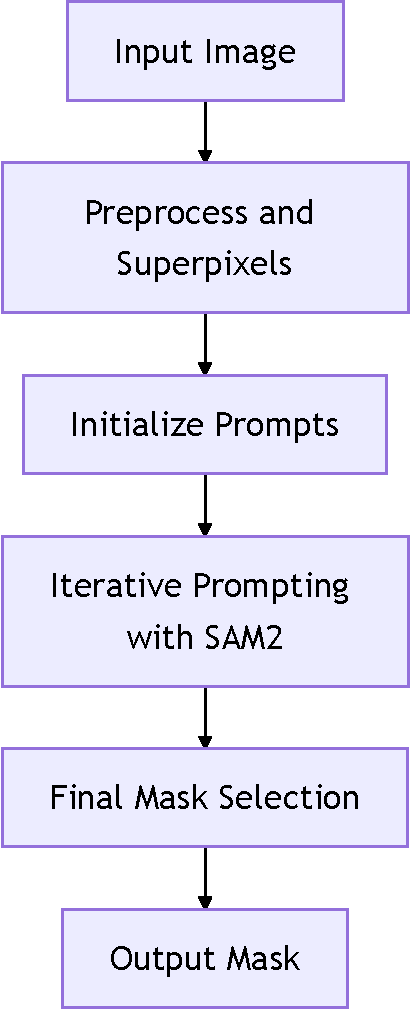
\includegraphics[width=\linewidth,height=0.85\textheight,keepaspectratio]{mermaid/pdfs/flow_overview.pdf}
  \caption{Main SGIP flow}
\end{figure}
\newpage

\subsection*{Step 1 — Preprocess \& Superpixels}
\begin{enumerate}[leftmargin=1.25em]
  \item \textbf{Input Image:} start from $I$.
  \item \textbf{Resize Long Side:} $I' \leftarrow \mathrm{ResizeLongSide}(I, L)$.
  \item \textbf{SLIC Superpixels:} $S \leftarrow \mathrm{SLIC}(I', K, c)$ in RGB space.
  \item \textbf{Compute Superpixel Sets $\Omega_j$:} $\Omega_j \leftarrow \{x \mid S(x)=j\}$.
  \item \textbf{Compute Centroids $\mu_j$:} $\mu_j \leftarrow c(\Omega_j)$ (deterministic placement).
  \item \textbf{Compute Intensity Proxy $g_j$:} $g_j \leftarrow \frac{1}{|\Omega_j|}\sum_{x\in\Omega_j} \mathrm{Gray}(I'(x))$.
\end{enumerate}

\begin{figure}[H]
  \centering
  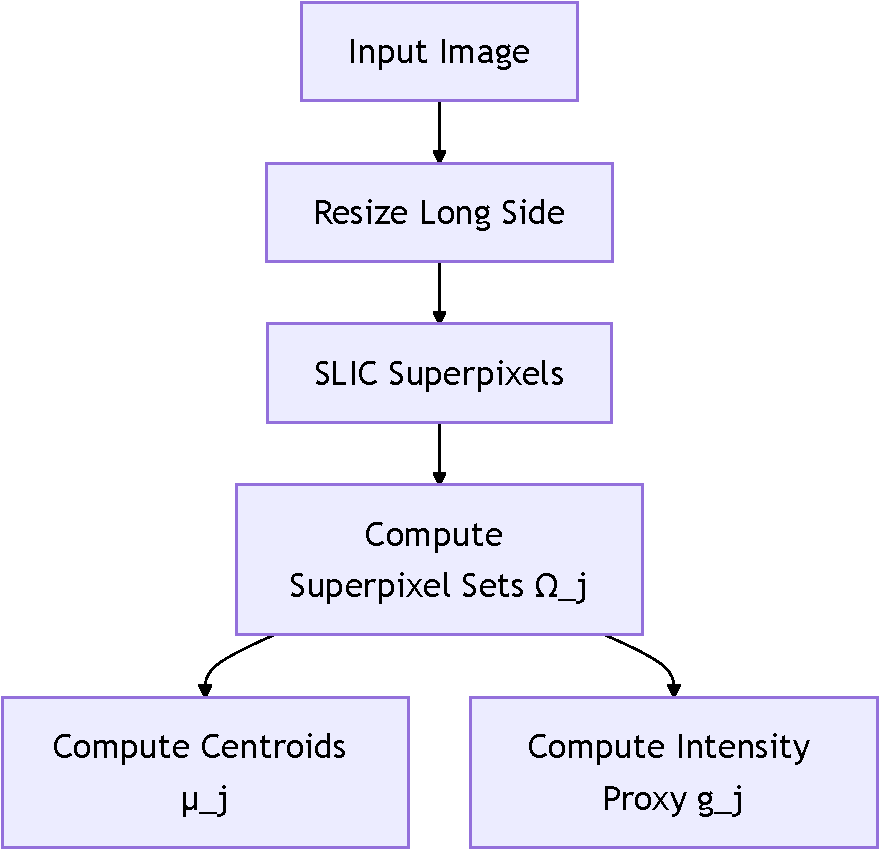
\includegraphics[width=\linewidth,height=0.85\textheight,keepaspectratio]{mermaid/pdfs/flow_preprocess.pdf}
  \caption{Preprocess \& superpixels}
\end{figure}
\newpage

\subsection*{Step 2 — Initialize Prompts}
\begin{enumerate}[leftmargin=1.25em]
  \item \textbf{Superpixels $\mu_j$ and $g_j$:} use centroids and intensity proxies from Step 1.
  \item \textbf{Select Center-Window Superpixels:} $\mathcal{C} \leftarrow \{ j \mid \mu_j^{\text{norm}} \in [\alpha,1-\alpha]^2 \}$.
  \item \textbf{Sort by Intensity Proxy $g_j$ (center):} sort $\mathcal{C}$ by $g_j$ descending.
  \item \textbf{Select Top $n_+$ as Positive Seeds:} $\mathcal{J}_+ \leftarrow$ first $n_+$ indices.
  \item \textbf{Add Positive Prompts:} $P \leftarrow \{(\mu_j, +1)\mid j\in\mathcal{J}_+\}$.
  \item \textbf{Select Boundary Superpixels:} $\mathcal{B} \leftarrow \{ j \mid \Omega_j \cap \partial\Omega \neq \varnothing \}$.
  \item \textbf{Sort by Intensity Proxy $g_j$ (boundary):} sort $\mathcal{B}$ by $g_j$ descending.
  \item \textbf{Select Top $m_-$ as Negative Seeds:} $\mathcal{J}_- \leftarrow$ first $m_-$ indices.
  \item \textbf{Add Negative Prompts:} $P \leftarrow P \cup \{(\mu_j, -1)\mid j\in\mathcal{J}_-\}$.
  \item \textbf{Initialize Prompt Set $P$:} maintain \texttt{PosIdx} and \texttt{NegIdx}.
  \item \textbf{Initialize Mask Prompt Empty:} $M^{\text{prompt}} \leftarrow \mathbf{0}$.
  \item \textbf{Initialize Candidate Pool $Q$ Empty:} $\mathcal{Q} \leftarrow [\ ]$.
\end{enumerate}

\begin{figure}[H]
  \centering
  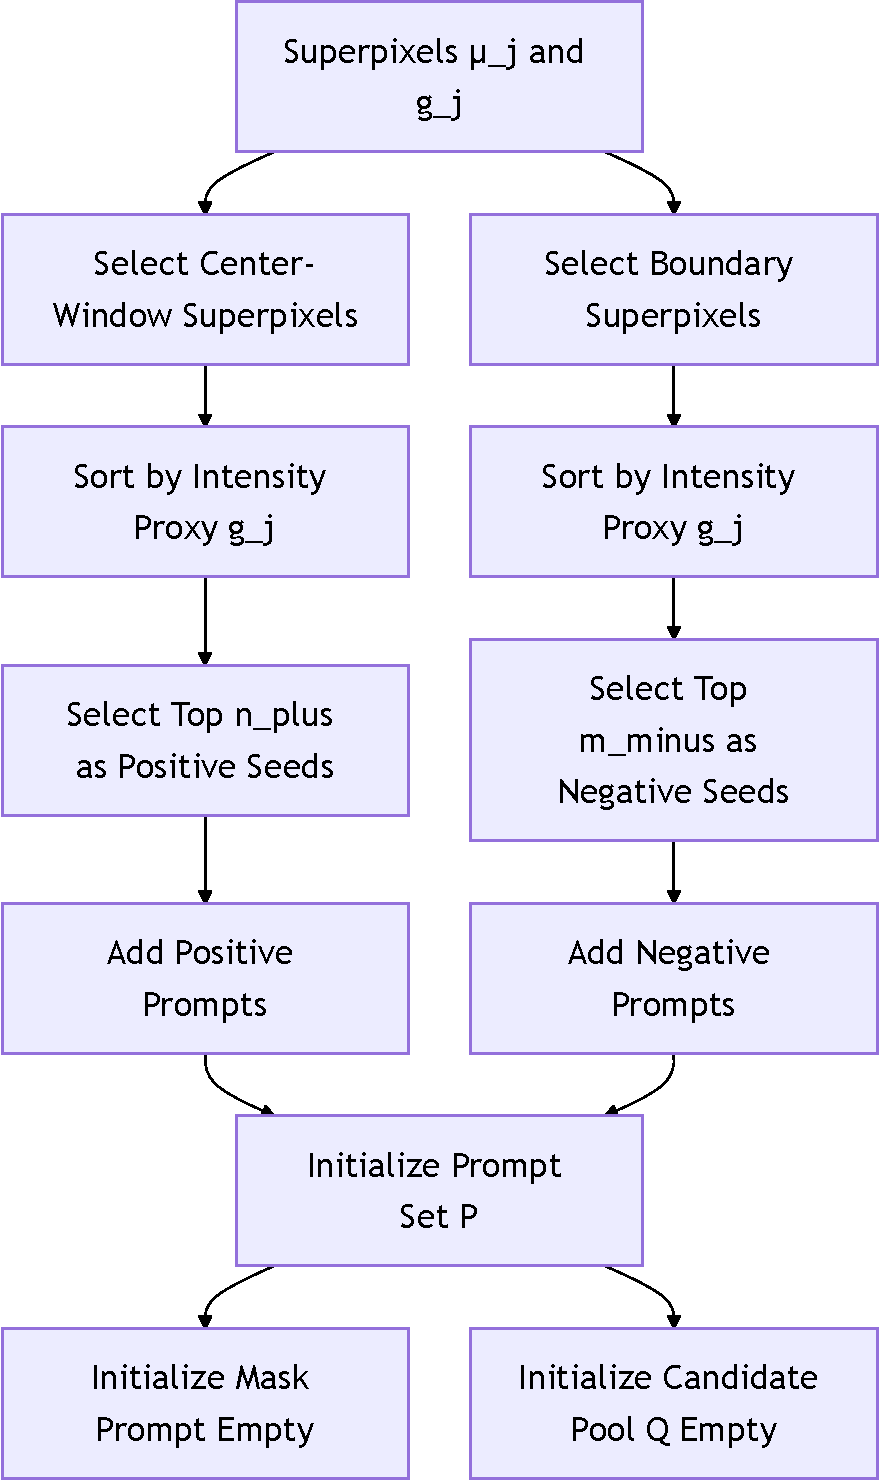
\includegraphics[width=\linewidth,height=0.85\textheight,keepaspectratio]{mermaid/pdfs/flow_init_prompts.pdf}
  \caption{Initialize prompts}
\end{figure}
\newpage

\subsection*{Step 3 — Iterative Prompting with Candidate Evaluation}
For $t = 1,2,\dots,T$:
\begin{enumerate}[leftmargin=1.25em]
  \item \textbf{Current Prompts and Mask:} use the current $P$ and $M^{\text{prompt}}$.
  \item \textbf{Generate Superpixel Scores:}
  \[
    (\ell_t, M_t, s_t) \leftarrow \mathrm{SAM2}(I', M^{\text{prompt}}, P),\quad
    p_t \leftarrow \sigma(\ell_t)
  \]
  \[
    v_j = \frac{1}{|\Omega_j|}\sum_{x\in\Omega_j} \ell_t(x),\quad j \notin (\texttt{PosIdx}\cup\texttt{NegIdx})
  \]
  \item \textbf{Select and Add Best Candidate:} select top-$q$ candidates, evaluate each with an extra positive point $(\mu_j,+1)$, choose $j^\star$ by highest score, and update $P$ and \texttt{PosIdx}.
  \item \textbf{Point placement note:} when adding a prompt for a region $R$, use its centroid $c(R)$ if $c(R)\in R$; otherwise use the nearest pixel in $R$ to $c(R)$. This avoids centroid-outside-region issues.
  \item \textbf{Optional Convex Hull / Pruning:} apply selective convex hull and/or prune close positives.
  \item \textbf{Update Mask Prompt + Append to Pool:}
  \[
    M^{\text{prompt}} \leftarrow \left( \bigcup_{(u,+1)\in P} \Omega_{S(u)} \right),\quad
    \mathcal{Q}.\text{append}((M_t, s_t))
  \]
  \item \textbf{More Valid Candidates?} stop if none remain.
\end{enumerate}


\begin{figure}[H]
  \centering
  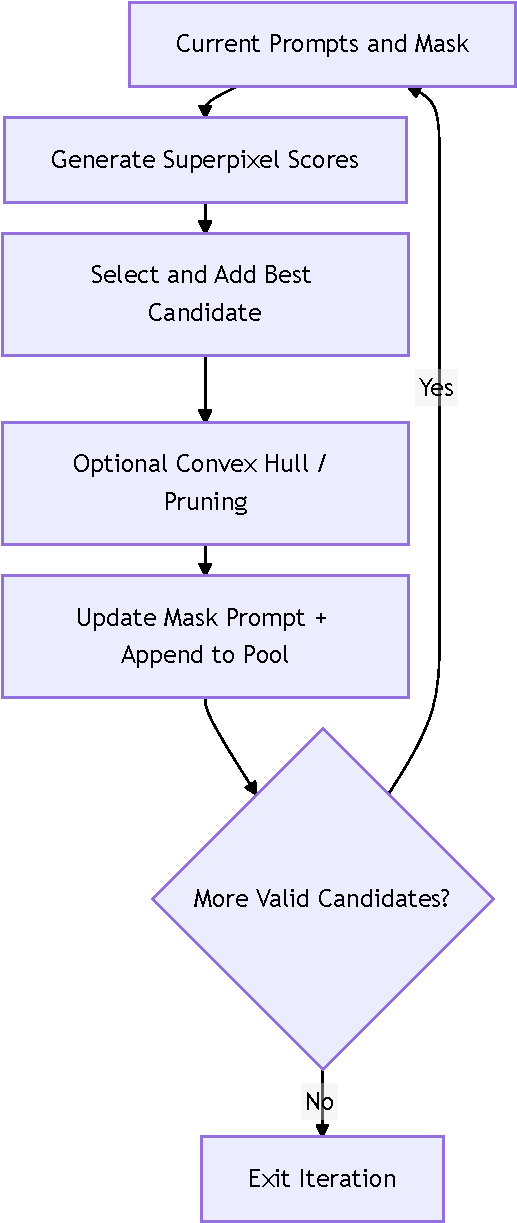
\includegraphics[width=\linewidth,height=0.85\textheight,keepaspectratio]{mermaid/pdfs/flow_iterative_prompting.pdf}
  \caption{Iterative prompting with candidate evaluation}
\end{figure}
\newpage

\subsubsection*{Step 3.1 — Candidate Pool Evaluation (\texttt{evaluate\_candidates})}
\begin{enumerate}[leftmargin=1.25em]
  \item \textbf{Valid candidate set $U$:} unlabeled, non-boundary superpixels.
  \item \textbf{Compute $v_j$:} score each candidate by mean logit in its superpixel.
  \item \textbf{Select Top-$q$ candidates $K$:} $q=\texttt{candidate\_top\_k}$.
  \item \textbf{Evaluate each $j \in K$:} run SAM2 with $(\mu_j,+1)$ and record $s^{(j)}$.
  \item \textbf{Pick best candidate:} choose $j^\star$ with highest $s^{(j)}$ and keep its mask $M_t$.
\end{enumerate}

\begin{figure}[H]
  \centering
  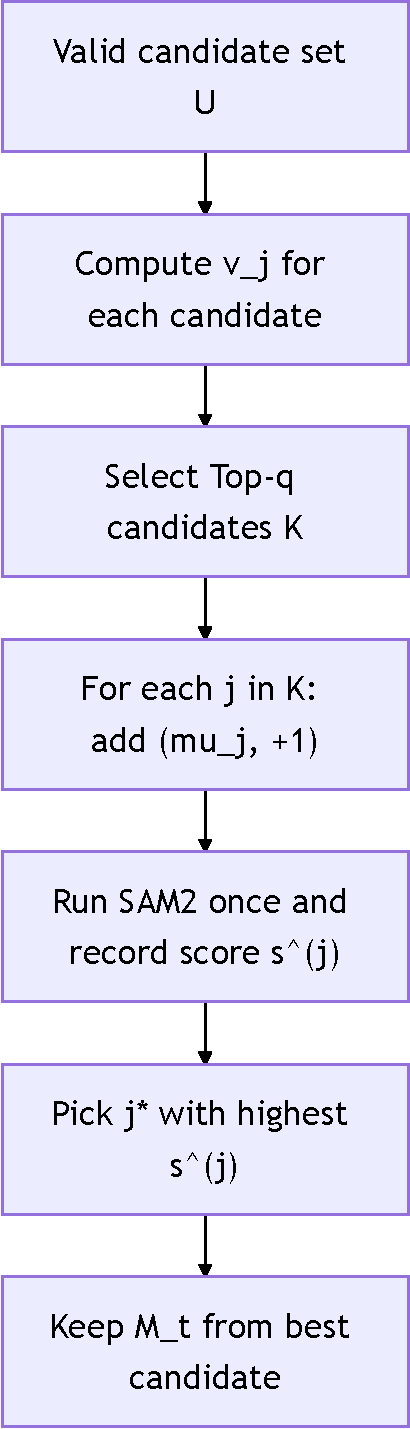
\includegraphics[width=\linewidth,height=0.85\textheight,keepaspectratio]{mermaid/pdfs/flow_candidate_pool.pdf}
  \caption{Candidate pool evaluation}
\end{figure}
\newpage

\subsection*{Step 4 — Final Mask Selection}
Let candidates be $\{(M_i, s_i)\}_{i=1}^{N}$ from $\mathcal{Q}$.
\begin{enumerate}[leftmargin=1.25em]
  \item \textbf{IoU De-duplication:} if $\mathrm{IoU}(M_a, M_b) > \tau_{\text{iou}}$, keep the higher-score mask.
  \item \textbf{Remaining Masks $\ge 3$?} if not, return $M^\star = \arg\max_i s_i$.
  \item \textbf{Cluster Masks by Area:} $k=3$ with centers at $\min(a)$, $\mathrm{median}(a)$, and $\max(a)$.
  \item \textbf{Select Middle Cluster:} choose $C_{\text{mid}}$ by centroid area.
  \item \textbf{Pick Max-Score Mask:} $M^\star = \arg\max_{M_i \in C_{\text{mid}}} s_i$.
\end{enumerate}

\begin{figure}[H]
  \centering
  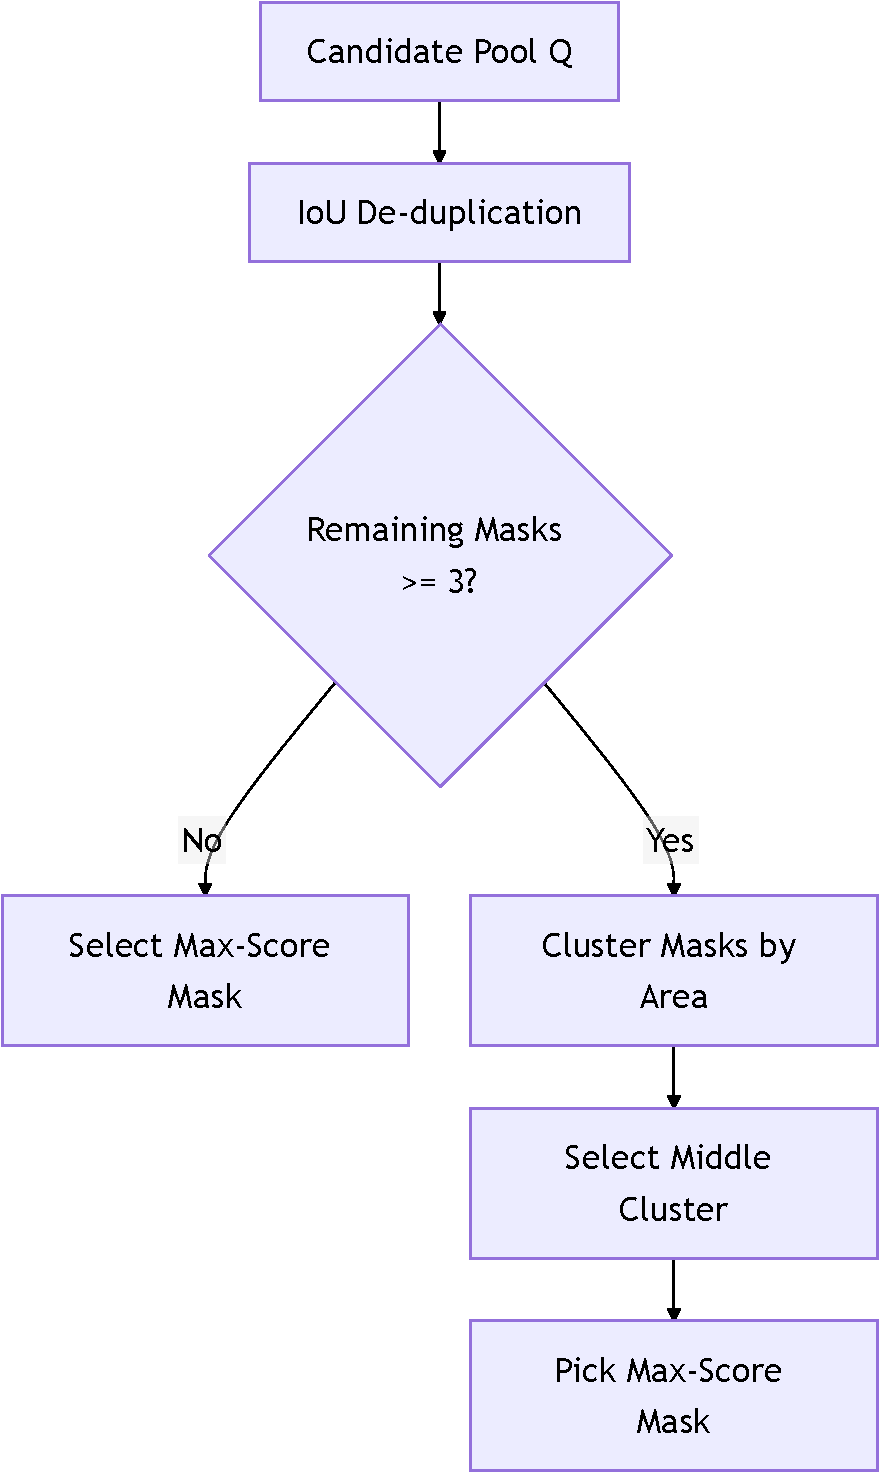
\includegraphics[width=\linewidth,height=0.85\textheight,keepaspectratio]{mermaid/pdfs/flow_final_selection.pdf}
  \caption{Final mask selection}
\end{figure}
\newpage

\section*{Output}
Final mask $M^\star$.

\end{document}
